\section{Construction of the NINJA-2 data set}


In broad terms the plans for the NINJA-2 data sets follow those for
NINJA-1 (ch.~\ref{ch:ninja1}).  Simulated Gaussian noise was generated
to model the initial LIGO and Virgo noise curves, the spectra are
identical to those in figure~\ref{f:ninjapsd}.  Injection parameters,
including choice of waveform, were then selected randomly.  The
injections were then added to the Gaussian noise and distributed to
data analysis groups.  However, several key changes were made in the
details of this process in order to correct shortcomings in NINJA-1.  

The NINJA-2 data was sampled at 16384 Hz rather than the 4096 Hz used
by NINJA-1.  This was done because investigations showed that there is
power above 4096 Hz in the waveforms, which would get aliased down to 
lower frequencies if the sample rate is too low.  This problem is
illustrated in figure~\ref{f:ninja2_aliasing}.

\begin{figure}
  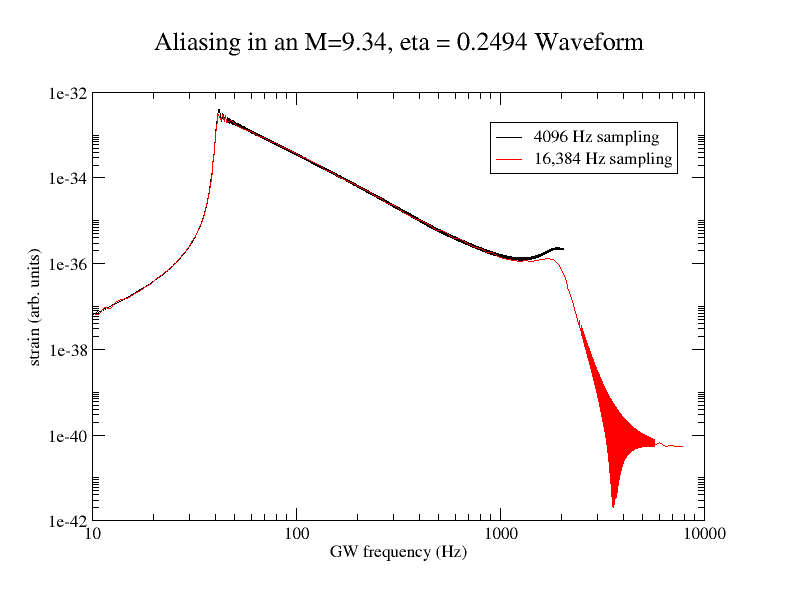
\includegraphics[width=\linewidth]{figures/ninja2_results/ninja2_aliasing}
  \caption[Aliasing of waveform power]{
  \label{f:ninja2_aliasing}
Frequency-domain amplitudes of a NINJA-2 waveform at different
sampling rates.  At a sample rate of 4096 Hz the late portion of the
waveform are distorted due to aliasing of power to lower frequencies.
}
\end{figure}%

NINJA-1 consisted of only 127 injections in a day of data, which
severely limited the ability to draw statistical conclusions on the
behavior of the pipelines.  To correct this in NINJA-2 we extended the
duration to eight weeks.  The density of injections was varied over
this span:  weeks 1-3 had one injection on average every 2000 seconds,
week 4-6 had one injection on average every 14,400 seconds, and the
final two weeks had one injection every on average every 216,000
seconds.  The intent was that data analysts can tune and test their
pipelines on the dense weeks, and then optionally perform a
self-blinded test on the final two weeks.

In NINJA-1 the SNR was not chosen a priori but was determined by the
other parameters.  For NINJA-2 we draw the network SNR ($\sqrt{\sum_i
\rho_i^2}$ where $i$ ranges over the IFOs) from a distribution and
then scale the distance of the injection in order to achieve that SNR.
For the first three weeks the distribution is linear from 6 to 130 in
order to allow pipelines to test and tune out to large SNRs on the
densest set of injections.  For the remaining weeks the distribution
falls as the reciprocal of the network SNR (uniform in
$\log(\mathrm{SNR})$) in order to better model the expected
astrophysical distribution.

The mass and waveform selection were also done slightly differently in
NINJA-2.  For each injection a mass was first selected uniformly over
the specified range; for the full 2-month run this range is from
$10-350 \msun$.  Then waveforms were selected at random until one was
found that could be injected at the chosen mass such that the waveform
turns on below 35 Hz.  In practice this condition never caused any
waveform to be rejected, as all submitted waveforms were long enough
to be injected down to the lowest mass in the range.  The mass ratio
and spins are intrinsic to the waveforms, so choosing a submission
amounts to a choice of these parameters as well.  A plot of the
selected masses, spins, and distances in the two-month run is shown in
figure~\ref{f:ninja2_dataset}.

\section{Test one-week Gaussian data set}

\begin{figure}
  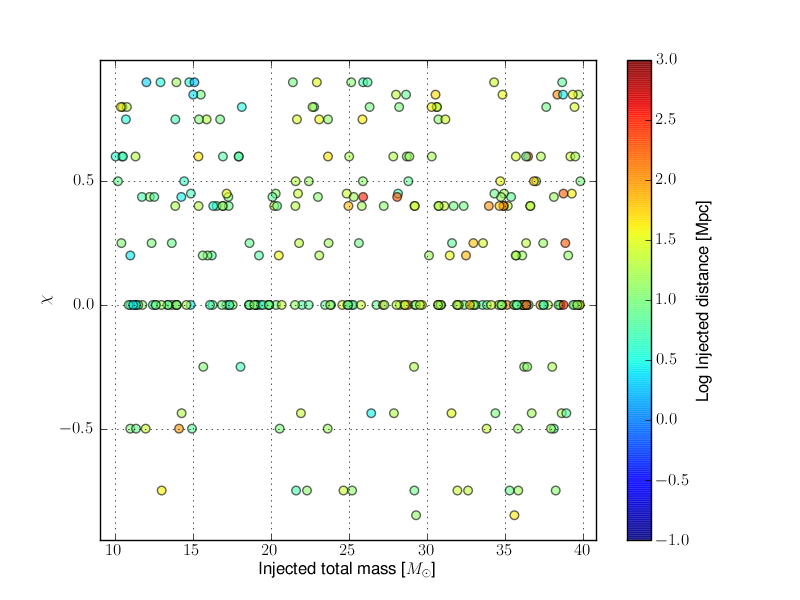
\includegraphics[width=\linewidth]{figures/ninja2_results/ninja2_test_dataset.png}
  \caption[Parameters of the NINJA-2 test one-week data set]{
  \label{f:ninja2_test_dataset}
Distribution of mass, spin and distance parameters in the one-week,
Gaussian-noise test data set.
}
\end{figure}%

\begin{figure}
  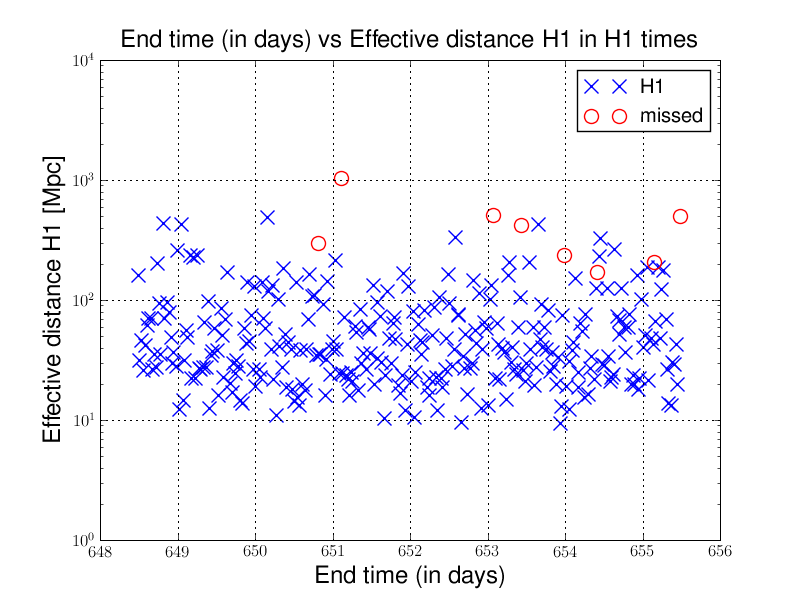
\includegraphics[width=0.5\linewidth]{figures/ninja2_results/h1-plotinspmissed_full_data_time-eff_dist-log-h1-871147524-606064.png}
  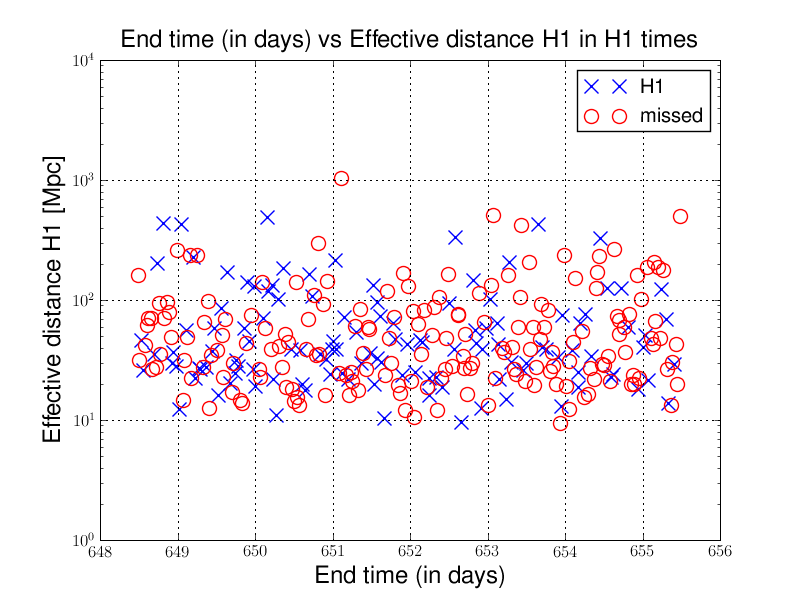
\includegraphics[width=0.5\linewidth]{figures/ninja2_results/h1-plotinspmissed_full_data_time-eff_dist-log-h1-871147524-606064_noiseonly.png} \\
  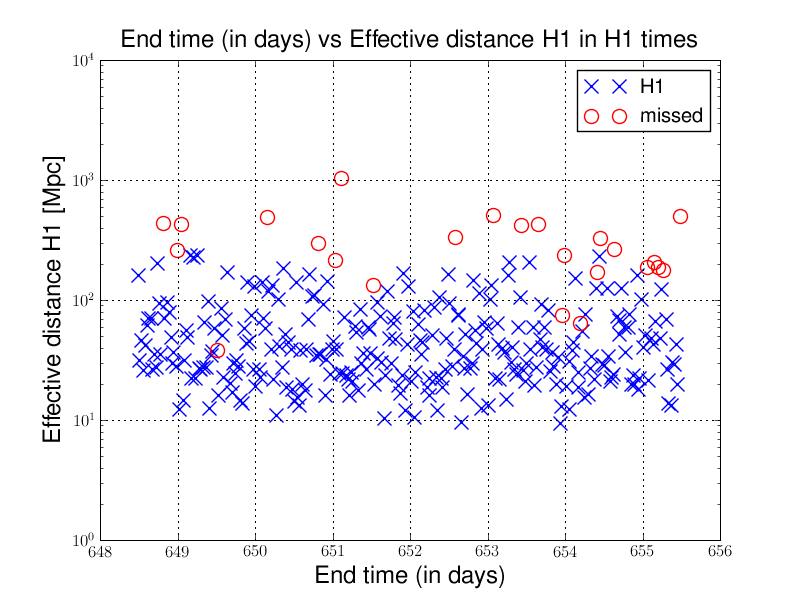
\includegraphics[width=\linewidth]{figures/ninja2_results/h1-plotinspmissed_full_data_time-eff_dist-log-h1-871147524-606064_second.png}
  \caption[First- and second-stage triggers from the test data set]{
  \label{f:first_and_second}
\Note{Explain the importance of looking at second-stage triggers when
determining what is actually ``found'', even in Gaussian noise.}
}
\end{figure}%


\begin{figure}
  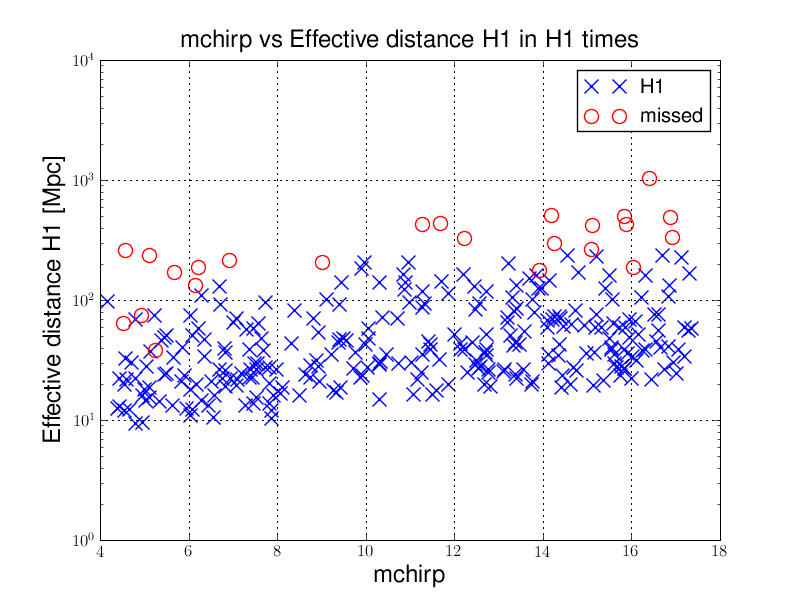
\includegraphics[width=0.5\linewidth]{figures/ninja2_results/h1-plotinspmissed_full_data_mchirp-eff_dist-log-h1-871147524-606064_second}
  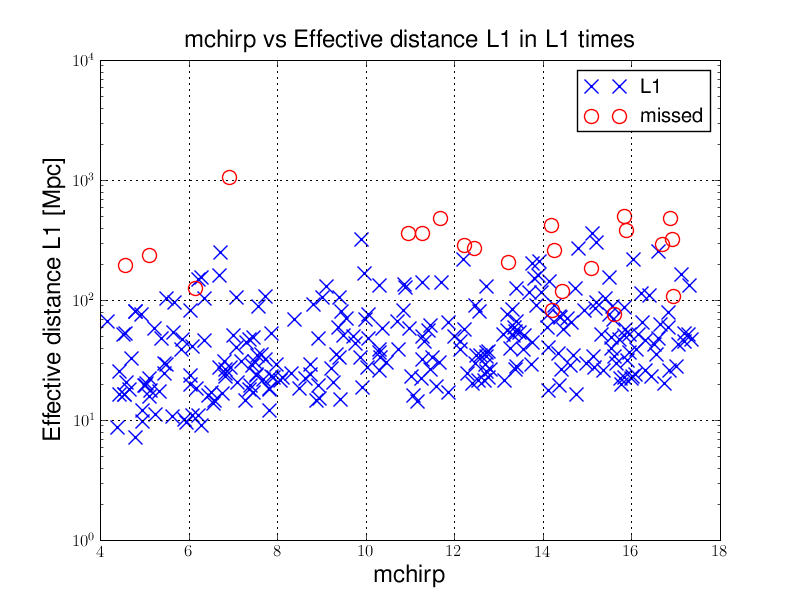
\includegraphics[width=0.5\linewidth]{figures/ninja2_results/l1-plotinspmissed_full_data_mchirp-eff_dist-log-l1-871147524-606064_second} \\
  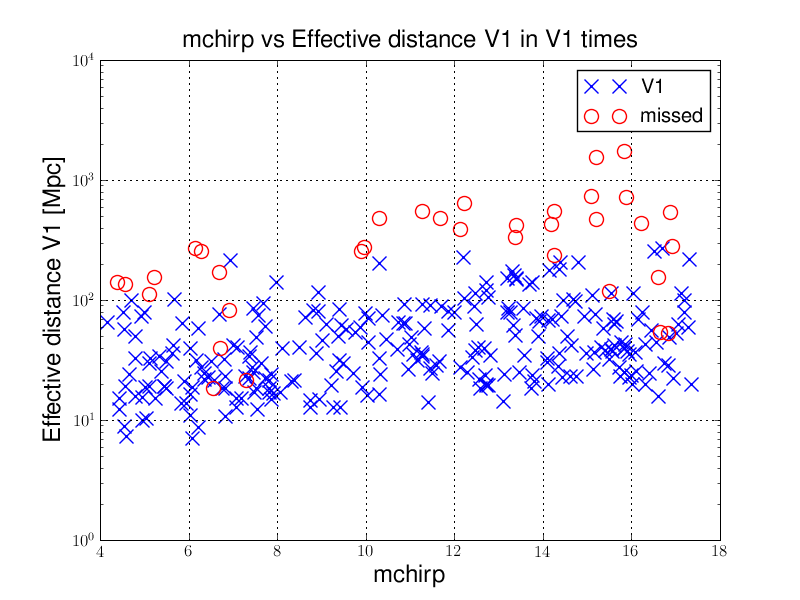
\includegraphics[width=\linewidth]{figures/ninja2_results/v1-plotinspmissed_full_data_mchirp-eff_dist-log-v1-871147524-606064_second}
  \caption[Found/missed plots for the test data set]{
  \label{f:test_found_missed}
}
\end{figure}%


\begin{figure}
  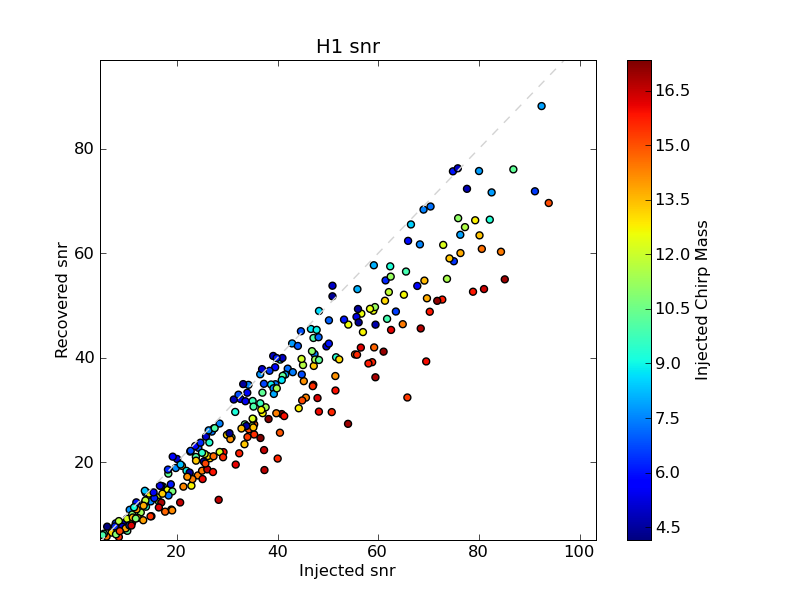
\includegraphics[width=0.5\linewidth]{figures/ninja2_results/h1_snrs_second}
  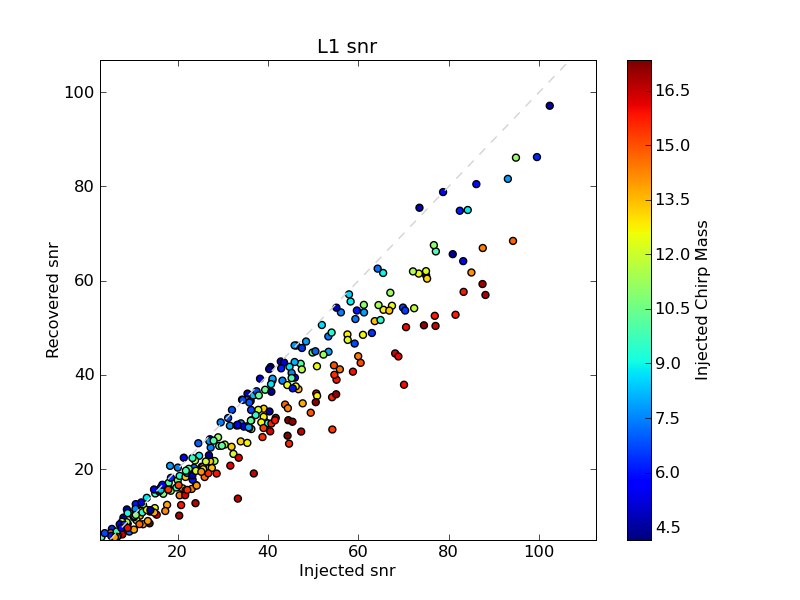
\includegraphics[width=0.5\linewidth]{figures/ninja2_results/l1_snrs_second} \\
  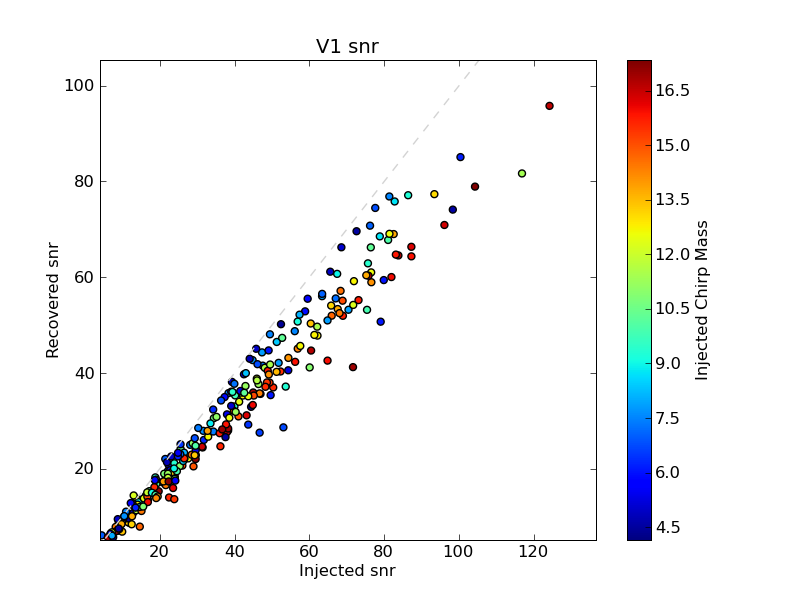
\includegraphics[width=\linewidth]{figures/ninja2_results/v1_snrs_second}
  \caption[SNR recovery for the test data set]{
  \label{f:test_recovered_snr}
}
\end{figure}%


\begin{figure}
  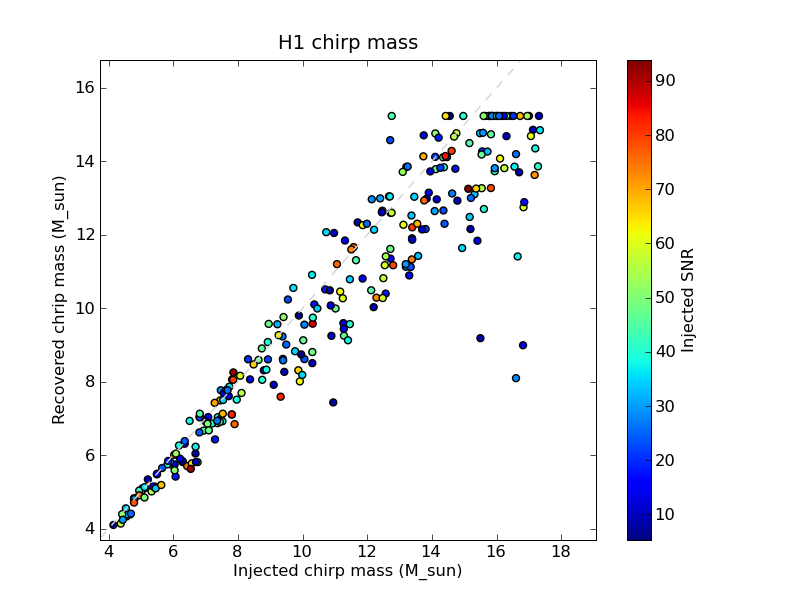
\includegraphics[width=0.5\linewidth]{figures/ninja2_results/h1_masses_second}
  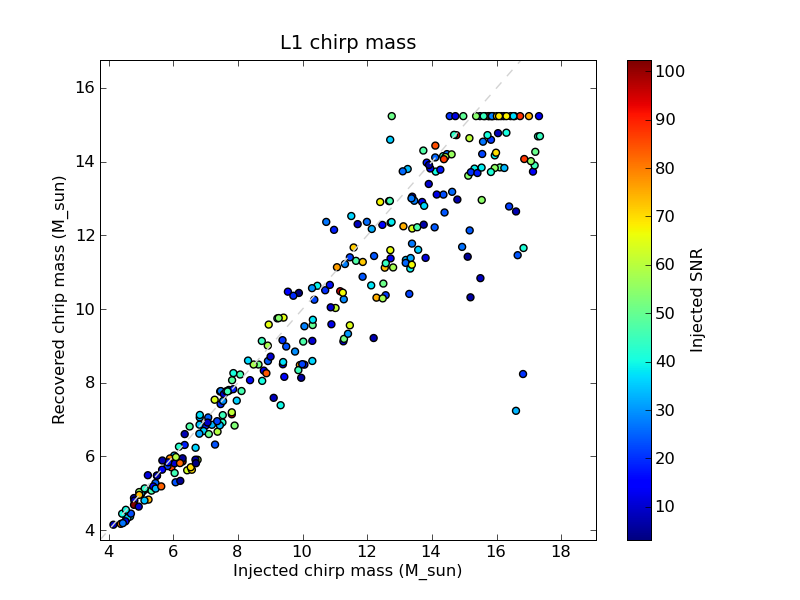
\includegraphics[width=0.5\linewidth]{figures/ninja2_results/l1_masses_second} \\
  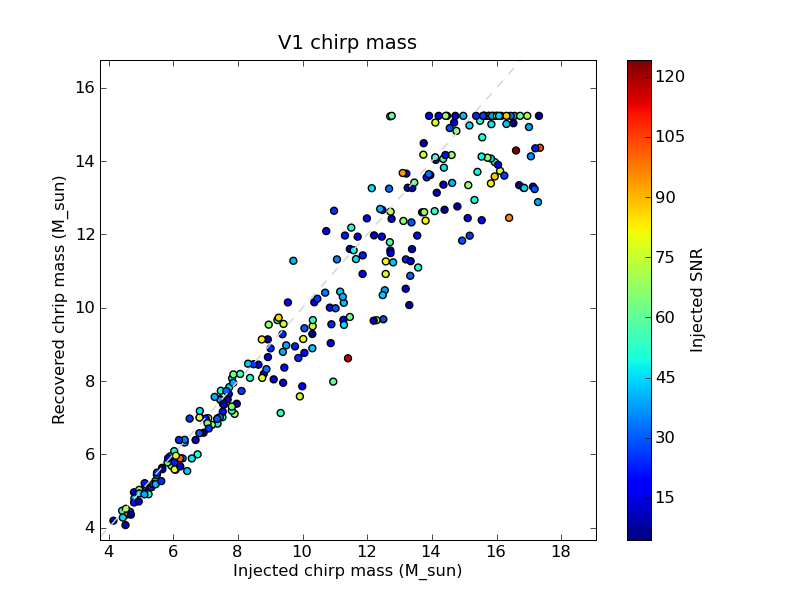
\includegraphics[width=\linewidth]{figures/ninja2_results/v1_masses_second}
  \caption[Mass recovery for the test data set]{
  \label{f:test_recovered_snr}
}
\end{figure}%


\section{Two-month Gaussian data set}

\begin{figure}
  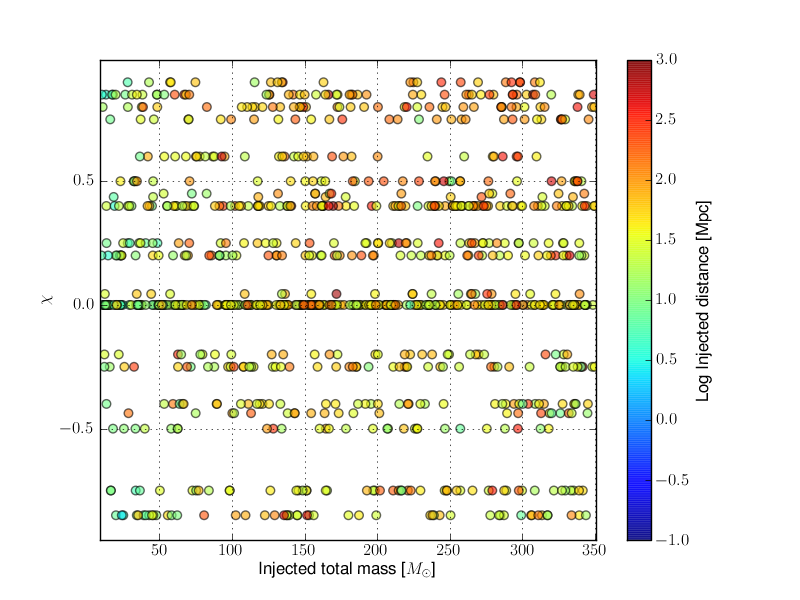
\includegraphics[width=\linewidth]{figures/ninja2_results/ninja2_dataset.png}
  \caption[Parameters of the NINJA-2 two-month data set]{
  \label{f:ninja2_dataset}
Distribution of mass, spin and distance parameters in the two-month,
Gaussian-noise data set.
}
\end{figure}%


As in NINJA-1 the sky location and inclination were chosen uniformly
at random.

For NINJA-2, in sharp contrast to NINJA-1, we created several two-week
test data sets in order to verify the waveforms and injection codes.
These tests were broken into smaller mass regions, ``low mass'' from
$10-40 \msun$, ``high-mass'' from $35-100 \msun$ and
``burst/ringdown'' from $80-350 \msun$.  The original intent had been
to create three full 2-month data sets along these same lines, but
that proved to be infeasible due to the file size of the data sets.
However, it was useful in the test sets as it allowed several
pipelines to do sanity checks in the mass region to which they are
most sensitive.  These tests exposed several bugs in the injection
codes which were fixed before generating the two-month data set.

\iffalse
Real detector data is far from Gaussian, and real data analysis is
concerned not only with foreground triggers from signals but also
background triggers from noise.  In order to comprehensively test the
ability of pipelines to detect signals and recover their parameters it
is necessary to perform injections into real detector noise.  As of
this writing a memorandum of understanding (MoU) between the NINJA
collaboration, the LIGO collaboration and the Virgo collaboration has
been signed which will allow subsequent NINJA-2 data sets to use data
from the previous (S5/VSR1) science run as noise.  A key feature of
this agreement is that NINJA is not a gravitational-wave search.  We
will therefore use data from disjoint periods in each instrument.
Details of this plan, such as which times to use, have yet to be
decided.  However it is clear we will need a custom segment database
(see chapter~\ref{ch:detchar}) to mark times where the instruments
were glitching. However, injection times will not use this
information, as it is entirely possible that real signals will land on
or near a glitch, and the ability to detect such signals is an
important test.
\fi

There are two motivations for constructing and distributing the data
sets as NINJA-1 and NINJA-2 thus far have done.  The first is to
ensure that every group is looking at the same set of injections so
that results can be compared.  The second is due to the terms of the
NINJA agreement, which restricted distribution of the raw NR
waveforms.  However, distribution of such static sets limits the
ability of individual groups to tune their pipelines in optimal ways,
and conceptually distributing a set of parameters would be sufficient
to compare results across pipelines.  In addition the size of the data
sets makes distribution slow and complex.  The NR groups within NINJA
have therefore relaxed the conditions on their use of their waveforms.
Consequently, subsequent NINJA-2 data sets will be distributed as sets
of parameters, and data analysis groups will use the available code to
either create data sets locally, or perform the injections ``on the
fly'' as the analysis is performed.  This will also allow groups to do
special-purpose tuning runs or analyses, the results of which may be
published as short-author papers subject to the conditions of the
NINJA agreement.


\subsection{CBC preliminary results}

The NINJA-2 data was analyzed with the standard CBC low-mass and
high-mass pipelines.  The parameters were exactly as in the S6/VSR2,3
runs, no changes were made to the configurations except for those
relating to the names of the data files.  The low-mass search uses
Taylor F2 templates to 3.5 pN order in phase evolution
(section~\ref{sec:PNWaveforms}) in a mass region defined by minimum component
masses of $1 \msun$ and maximum total mass of $25 \msun$.  The high
mass search uses EOBNR templates (section~\ref{ssec:EOB}) in a region
defined by minimum component masses of $1 \msun$, minimum total mass
of $25 \msun$, and maximum total mass of $100 \msun$.  Plots of found
and missed injections are shown in figure~\ref{f:ninja2_cbc_results}.

\begin{figure}
  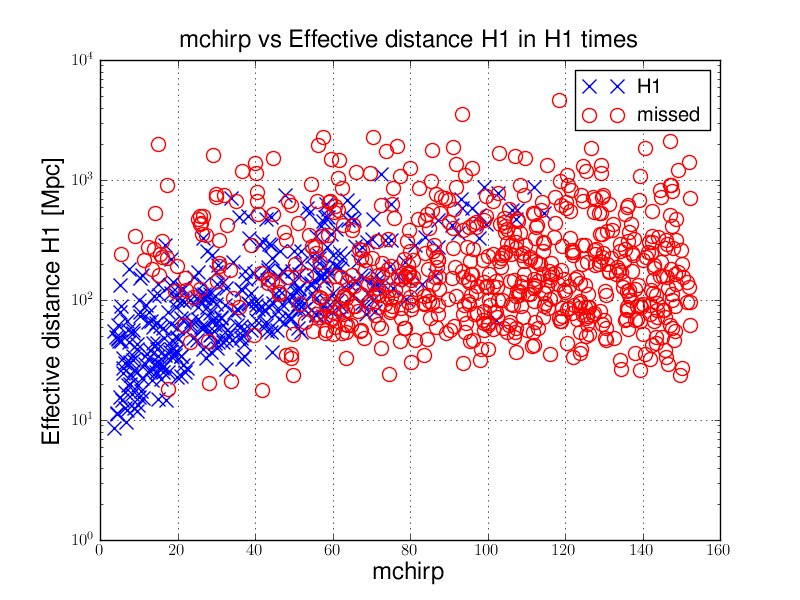
\includegraphics[width=0.5\linewidth]{figures/ninja2_results/H1-plotinspmissed_LOW_FULL_DATA_mchirp-eff_dist-log-H1-871147552-5209912.png}
  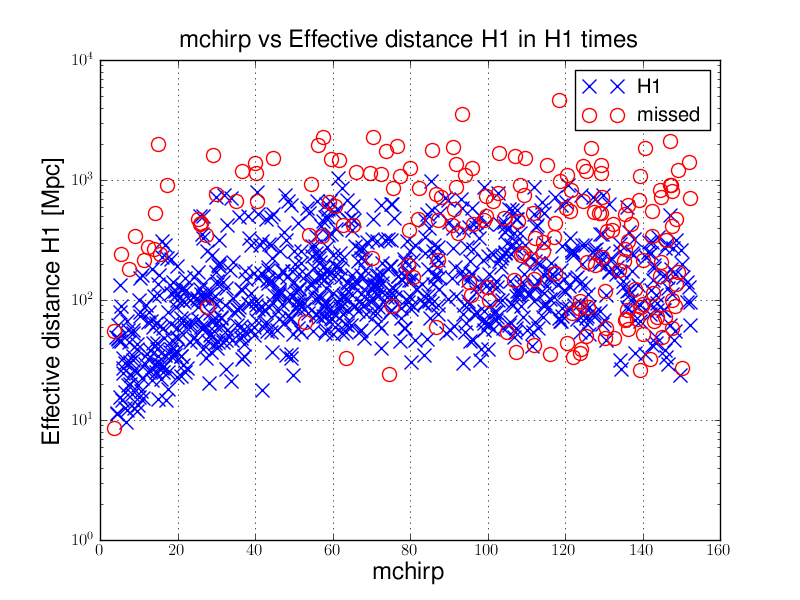
\includegraphics[width=0.5\linewidth]{figures/ninja2_results/H1-plotinspmissed_HIGH_FULL_DATA_mchirp-eff_dist-log-H1-871147552-5209912.png} \\
  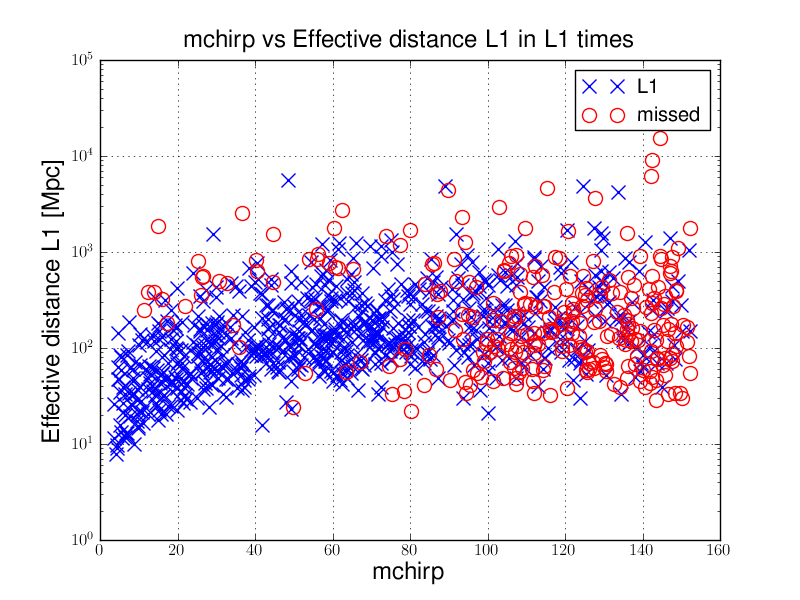
\includegraphics[width=0.5\linewidth]{figures/ninja2_results/L1-plotinspmissed_LOW_FULL_DATA_mchirp-eff_dist-log-L1-871147552-5209912.png}
  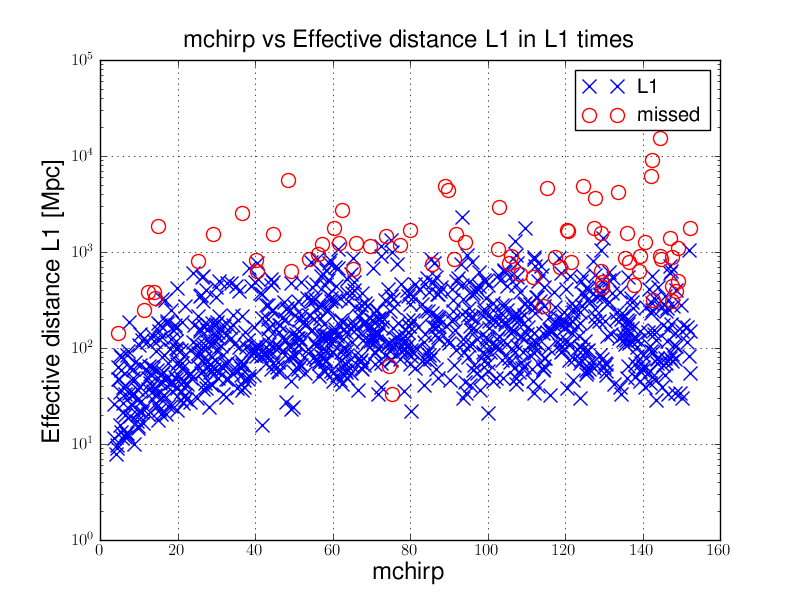
\includegraphics[width=0.5\linewidth]{figures/ninja2_results/L1-plotinspmissed_HIGH_FULL_DATA_mchirp-eff_dist-log-L1-871147552-5209912.png} \\
  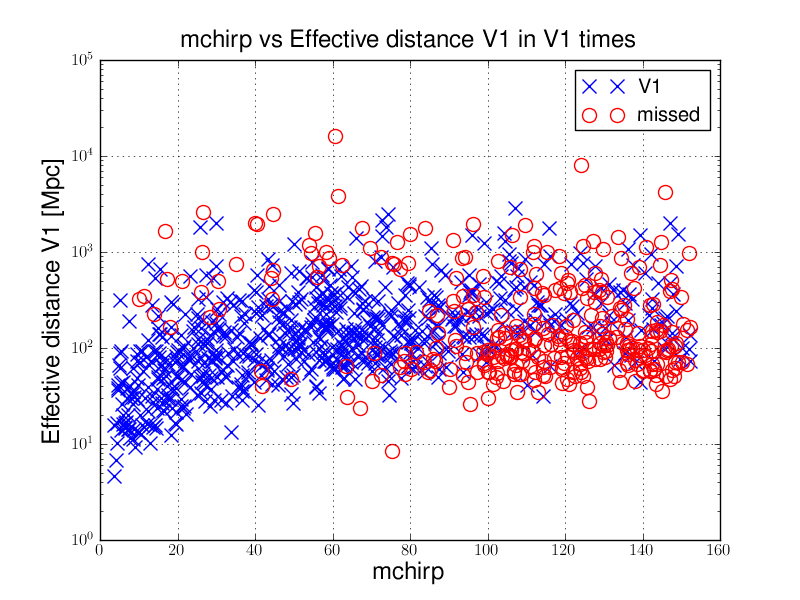
\includegraphics[width=0.5\linewidth]{figures/ninja2_results/V1-plotinspmissed_LOW_FULL_DATA_mchirp-eff_dist-log-V1-871147552-5209912.png}
  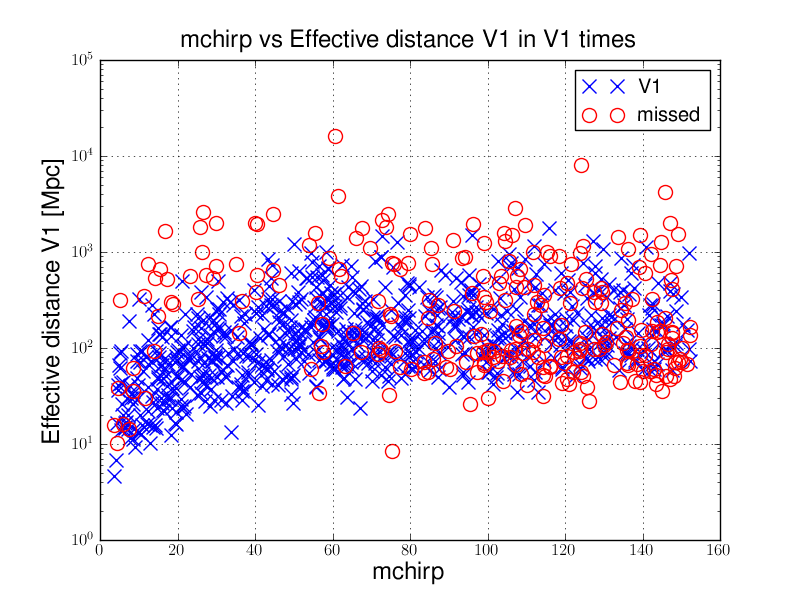
\includegraphics[width=0.5\linewidth]{figures/ninja2_results/V1-plotinspmissed_HIGH_FULL_DATA_mchirp-eff_dist-log-V1-871147552-5209912.png} \\
  \caption[Preliminary NINJA2 CBC results]{
  \label{f:ninja2_cbc_results}
Preliminary results from the CBC low-mass (left) and high-mass (right)
pipelines on the two-month NINJA-2 data set.
}
\end{figure}%


\noindent \Note{TODO: Show efficiency as a function of mass, for all
signals and just for non-spinning.}

\noindent \Note{TODO: explain anomalous Virgo results.}

